% !TeX root = main.tex
\section{Resultados}
\label{sec:resultados}

\subsection{Caso evaluado y primer corte}

Se presentan los resultados guardados en el cuaderno para
el caso \texttt{VS-SEG-001}~\cite{cuaderno}. La imagen contiene $512\times512$ píxeles y el
rectángulo seleccionado comprende 4958 píxeles. La referencia contiene
1690 píxeles positivos, todos dentro del rectángulo. El grafo reducido
incluye 4958 nodos variables y 19\,411 pares internos de vecinos; 278
píxeles interiores tienen conexiones con el fondo exterior. El parámetro
de contraste calculado sobre la imagen fue $\beta=0{,}001448$, con
$\gamma=10$.

El primer corte mínimo produjo una región de 1685 píxeles de primer plano.
La figura~\ref{fig:primer-corte} muestra la imagen y la segmentación dentro
del rectángulo. La región segmentada sigue la zona de mayor intensidad
asociada a la lesión. La proximidad entre su tamaño y el de la referencia
no establece por sí sola una coincidencia espacial, por lo que la
evaluación final considera las discrepancias píxel a píxel.

\begin{figure}[!htbp]
 \centering
 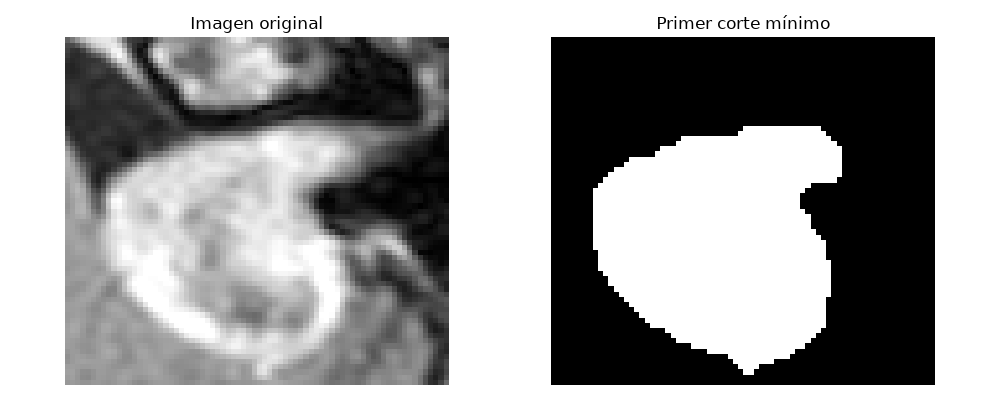
\includegraphics[width=0.95\textwidth]{vs-seg-001-primer-corte.png}
 \caption{Imagen de entrada y primer corte mínimo para
 \texttt{VS-SEG-001}, recortados al rectángulo seleccionado. El blanco
 representa el primer plano y el negro, el fondo en la segmentación.
 La región obtenida contiene 1685 píxeles. Figura exportada de la salida
 conservada en el cuaderno~\cite{cuaderno}; imagen de origen
 \cite{shapeydatos}.}
 \label{fig:primer-corte}
\end{figure}

\subsection{Evolución de la segmentación}

La primera iteración cambió 3273 etiquetas respecto de la inicialización,
en la que todos los píxeles interiores pertenecían al primer plano. La
segunda modificó 54 etiquetas y produjo una región de 1653 píxeles. Desde
la tercera hasta la quinta iteración no se registraron cambios en las
etiquetas. La tabla~\ref{tab:iteraciones} presenta las energías reducidas
antes y después de cada corte, calculadas con los modelos de esa iteración.

\begin{table}[!htbp]
 \centering
 \caption{Evolución de las cinco iteraciones para \texttt{VS-SEG-001}.
 Las energías corresponden a la ecuación~\eqref{eq:energia-reducida}.
 Cada comparación anterior--posterior utiliza los mismos parámetros
 gaussianos. Los valores se muestran con tres decimales.}
 \label{tab:iteraciones}
 \begin{tabular}{rrrr}
 \toprule
 Iteración & Etiquetas modificadas & Energía anterior & Energía posterior \\
 \midrule
 1 & 3273 & $33040{,}453$ & $29246{,}318$ \\
 2 & 54   & $28085{,}150$ & $28039{,}382$ \\
 3 & 0    & $28021{,}789$ & $28021{,}789$ \\
 4 & 0    & $28013{,}209$ & $28013{,}209$ \\
 5 & 0    & $27996{,}347$ & $27996{,}347$ \\
 \bottomrule
 \end{tabular}
\end{table}

La energía disminuyó durante los dos primeros cortes y permaneció igual
antes y después de los tres siguientes, a la precisión registrada.
Aunque las etiquetas no cambiaron en esas últimas iteraciones, la energía
varió entre ellas debido a la actualización de los modelos de intensidad.
La estabilidad observada corresponde a las etiquetas durante las cinco
iteraciones ejecutadas; no constituye una prueba de convergencia conjunta
de todos los parámetros.

\subsection{Comparación con la referencia}

La segmentación final presentó 47 falsos positivos y 84 falsos negativos,
para un total de 131 discrepancias. A partir de estos conteos y de los
1690 píxeles de referencia, se obtienen 1606 verdaderos positivos y 1653
píxeles clasificados como primer plano. La tabla~\ref{tab:evaluacion-caso}
compara el resultado con la predicción que asigna fondo a toda la imagen.

\begin{table}[!htbp]
 \centering
 \caption{Evaluación del caso \texttt{VS-SEG-001}. Los falsos positivos
 (FP) y falsos negativos (FN) se cuentan sobre la imagen completa.
 El error cuadrático medio (ECM) se calcula sobre 262\,144 píxeles para
 la imagen y sobre 4958 píxeles para el rectángulo.}
 \label{tab:evaluacion-caso}
 \begin{tabular}{lrrrr}
 \toprule
 Método & FP & FN & ECM global & ECM en el rectángulo \\
 \midrule
 GrabCut & 47 & 84 & $0{,}000500$ & $0{,}026422$ \\
 Todo fondo & 0 & 1690 & $0{,}006447$ & $0{,}340863$ \\
 \bottomrule
 \end{tabular}
\end{table}

El error de GrabCut equivale aproximadamente al $0{,}050$~\% de la
imagen y al $2{,}642$~\% del rectángulo. Frente a la predicción de todo
fondo, el número de discrepancias se redujo aproximadamente un
$92{,}25$~\%. Esta reducción se calcula con los conteos enteros, antes del
redondeo de las métricas. La referencia ocupa solo el $0{,}645$~\% de la
imagen, lo que explica que la predicción de todo fondo también presente
un error global pequeño pese a omitir completamente la lesión.

La figura~\ref{fig:evaluacion-final} muestra la anotación, la referencia,
la segmentación final y la distribución espacial de las discrepancias.
Los falsos positivos se observan principalmente en los extremos derecho
e inferior de la región, mientras que los falsos negativos aparecen en
porciones de su borde izquierdo e inferior. Predominan los píxeles de
lesión correctamente identificados en el interior. Las diferencias se
concentran en el límite de la región y no quedan descritas únicamente por
su área total.

\begin{figure}[!htbp]
 \centering
 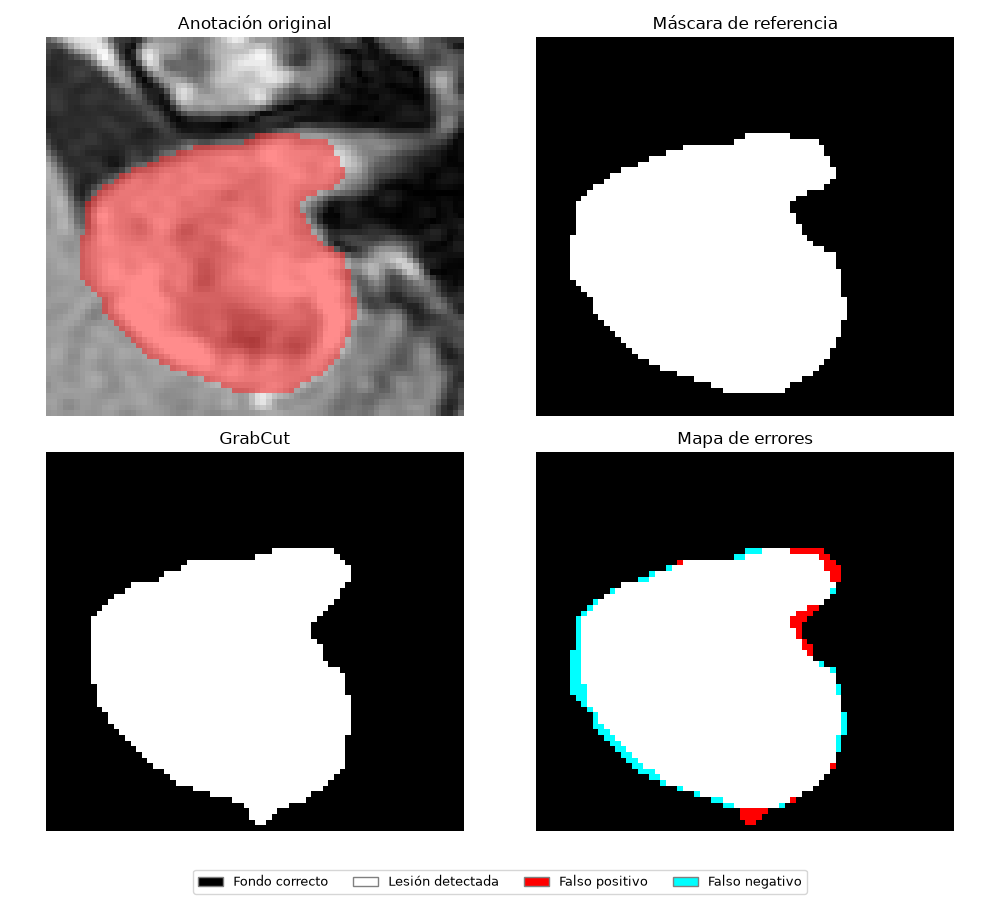
\includegraphics[width=0.86\textwidth]{vs-seg-001-evaluacion.png}
 \caption{Comparación final para \texttt{VS-SEG-001} dentro del rectángulo.
 Arriba: anotación roja y máscara binaria de referencia. Abajo:
 segmentación tras cinco iteraciones y mapa de errores. En este último,
 el blanco indica lesión correctamente identificada; el negro, fondo
 correcto; el rojo, falsos positivos; y el cian, falsos negativos.
 No hay píxeles de referencia fuera del rectángulo.
 Figura exportada de la salida conservada en el cuaderno~\cite{cuaderno}; imagen de origen
 \cite{shapeydatos}.}
 \label{fig:evaluacion-final}
\end{figure}

En el caso evaluado, la segmentación conservó la mayor parte de la región
anotada y las discrepancias se concentraron en sus bordes. Las etiquetas
se estabilizaron durante la ejecución, mientras continuaba el ajuste de
los modelos de intensidad.
